\documentclass[conference]{IEEEtran}
\IEEEoverridecommandlockouts
% The preceding line is only needed to identify funding in the first footnote. If that is unneeded, please comment it out.
\usepackage{cite}
\usepackage{amsmath,amssymb,amsfonts}
\usepackage{algorithmic}
\usepackage{subcaption}
\usepackage{graphicx}
\usepackage{textcomp}
\usepackage{xcolor}
\def\BibTeX{{\rm B\kern-.05em{\sc i\kern-.025em b}\kern-.08em
    T\kern-.1667em\lower.7ex\hbox{E}\kern-.125emX}}
\begin{document}

\title{A Deep Learning Project on Face Mask Detection\\}

\author{\IEEEauthorblockN{Abiha Tahsin Chowdhury}
\IEEEauthorblockA{\textit{Computer Science and Engineering} \\
\textit{AUST}\\
180104126@aust.edu}
\and
\IEEEauthorblockN{Barnana Prabeni Kristy}
\IEEEauthorblockA{\textit{Computer Science and Engineering} \\
\textit{AUST}\\
180104127@aust.edu}
\and
\IEEEauthorblockN{Shahajadi Sadia Afsana}
\IEEEauthorblockA{\textit{Computer Science and Engineering} \\
\textit{AUST}\\
180104138@aust.edu}
\and
\IEEEauthorblockN{Arpa Alam}
\IEEEauthorblockA{\textit{Computer Science and Engineering} \\
\textit{AUST}\\
180104143@aust.edu}
}

\maketitle

\begin{abstract}
Wearing a face mask is one of the numerous ways to stop the COVID-19 virus from spreading, and it is also one of the best ways to do it. During the coronavirus epidemic, face masks are worn by almost everyone at all times in public areas. This motivates us to investigate face mask recognition technologies to keep an eye on those who use masks in public. Tracking this policy's execution manually, however, is not practical. Here, technology is the key. We present a Deep Learning-based system that can identify situations in which face masks are improperly worn. Our approach is to use some deep learning architecture that can distinguish between faces that are covered with masks and those that are not. This will support the usage of face masks, track safety infractions, and guarantee a secure workplace.The proposed method correctly identifies the face in the picture or video, and then assesses whether or not it is wearing a mask. We look into the most effective parameter settings for some models in order to precisely detect the presence of masks. But keep in mind that wearing a mask won't be enough to stop the COVID-19 virus from spreading; we must all continue to keep our distance physically and constantly wash our hands. Together, these actions will help us defeat COVID-19.
\end{abstract}

\begin{IEEEkeywords}
 Mask, Picture, Deep Learning, Covid-19
\end{IEEEkeywords}

\section{Introduction}
To better understand the importance of wearing masks during the coronavirus pandemic, it is helpful to understand how the virus spreads. COVID-19 is currently thought to be spread primarily through close person-to-person contact, within about six feet, via respiratory droplets. When a person speaks, sneezes, coughs, or laughs, these tiny droplets are expelled from the nose and mouth. When droplets from a COVID-19-infected person land on an uninfected person's mouth or nose, he or she may contract the virus. As top health officials and scientists continue to learn more about the virus, it is now believed that asymptomatic individuals carrying the virus can also spread it through respiratory droplets.
\\
\\
The vaccine that can effectively treat Covid-19 has not yet been developed, and the globe has not yet fully recovered from this epidemic. However, numerous governments have permitted a small number of economic activities to be resumed once the number of new cases of Covid-19 has decreased below a particular level in an effort to lessen the pandemic's impact on the nation's economy. Concerns about workplace safety in the new post-Covid-19 climate have surfaced as these countries cautiously resume their economic operations.
\\
\\
It is recommended that people wear masks and keep a distance of at least one meter between each other to limit the risk of infection.Deep learning has attracted increased interest in the field of object detection and has been utilized to construct a face mask detection tool that can determine whether or not a person is wearing a mask. Real-time streaming from the Camera can be examined to evaluate the classification results. We require a training data collection for deep learning projects. It is the real data-set that was used to train the model to carry out different tasks.
\\
\\
Therefore, the major goal of our project is to identify faces in images and determine whether or not people are wearing masks at the time they are shot.

\section{Related Works}

\subsection{An Automated System to Limit COVID-19 Using Facial Mask Detection in Smart City Network\cite{b1}}

The brand-new coronavirus that sparked the COVID-19 epidemic is still circulating today. One of the many precautions used to halt the spread of this disease is wearing a mask. Our research may be able to assist various countries worldwide in halting the development of this dangerous illness. Using test data that had never been seen before, the trained architecture differentiated between people wearing facial masks and people wearing none with 98.7\% accuracy.

\subsection{Masked Face Recognition Using convolutional Neural Network\cite{b2}}
This study's primary objective is to increase the recognition precision of diverse masked faces, with a particular emphasis on facial masks. It has been proposed that a practical approach starts with the localization of the face areas. The difficult task of identifying faces in occluded situations has been taken on by a multi-task cascading convolutional neural network (MTCNN). The next step is to extract facial features using the Google Face Net embedding model.

\subsection{Face mask recognition system using CNN model\cite{b3}}
P. Gupta, N. Saxena, M. Sharma, and J. Tripathi (2018) suggest a novel approach for using a deep neural network in their study on facial recognition. This suggested method only employs the recovered facial features as input, as opposed to using raw pixel data. The proposed method does not compromise the framework's accuracy because it yields average accuracy of 97.05\%.

\section{Research Methodology}
We used python script,tensor flow,and some deep learning architectures to develop an efficient network for recognising face masks.The implementation of the project is carried out in python notebook. Libraries like pandas, NumPy, matplotlib, sklearn, etc. are used.Our objective is to train a specialised models to detect whether someone is wearing a mask or not.This project can instantly recognise the faces of the mask from any angle.It generates output from an RGB input image of any orientation.
Here is a flowchart of Methodology :

\begin{figure}[htbp]
        \centerline{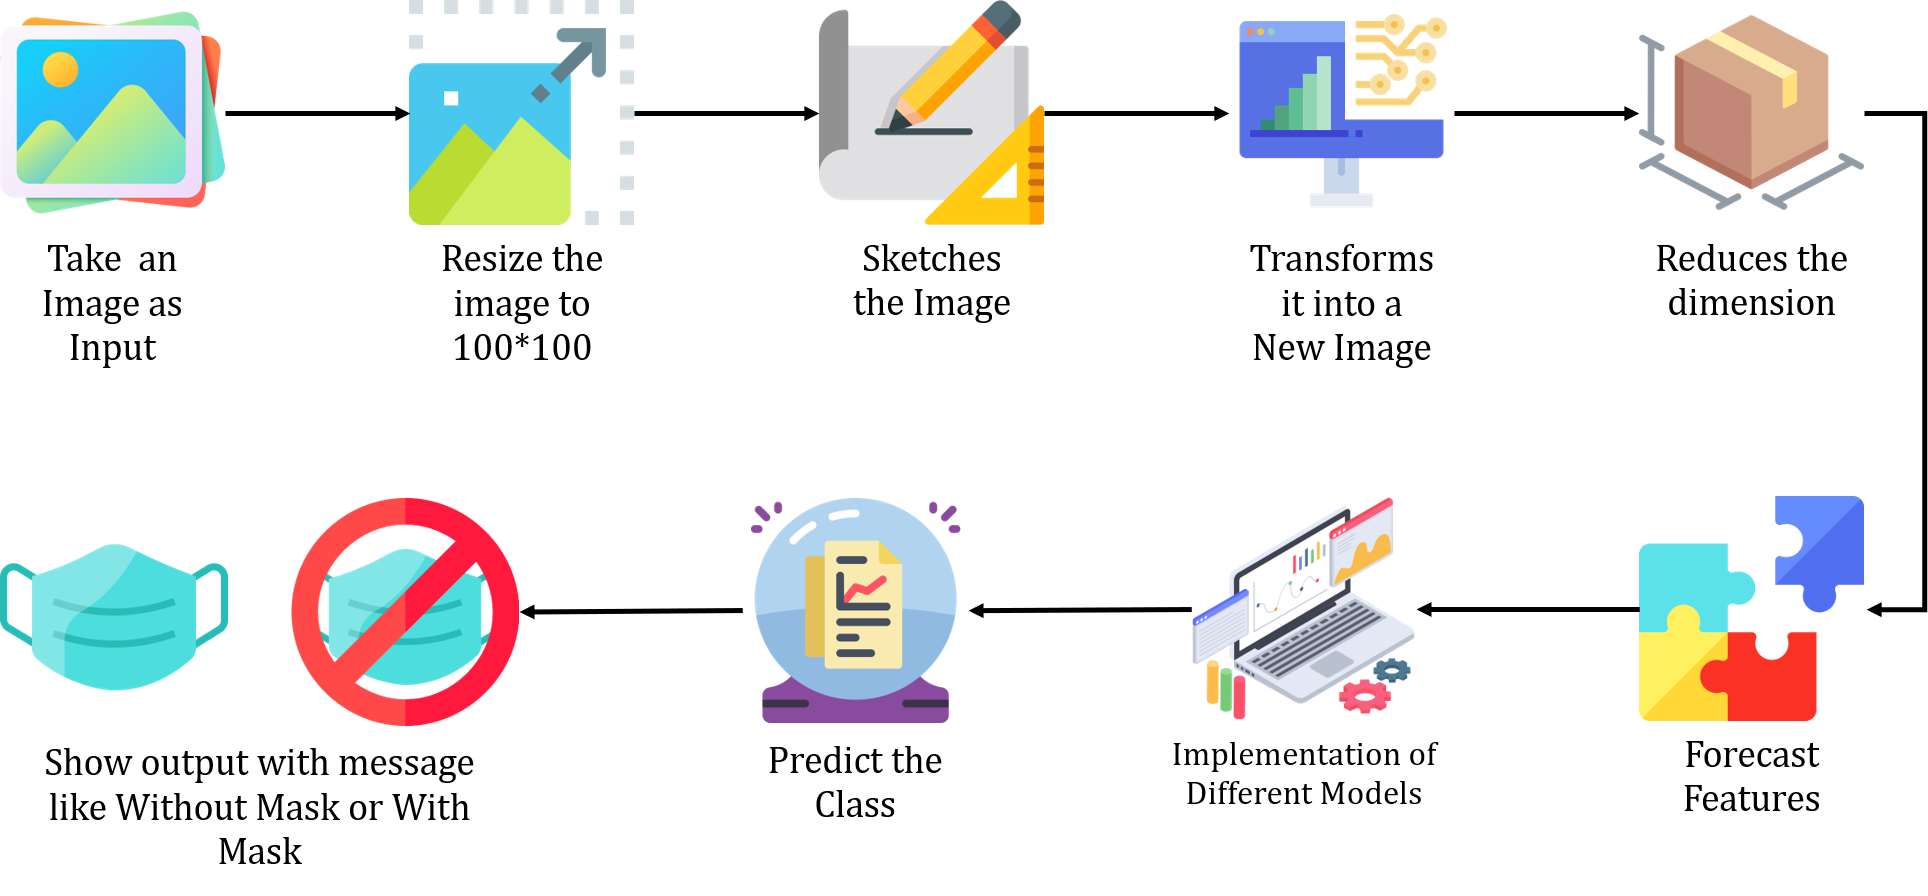
\includegraphics[width=9cm]{SC Flowchart2.png}}
        \caption{Flowchart of Methodology}
        \label{flowchart}
    \end{figure}


\section{Dataset}
For datasets we have used \textbf{Face Mask Detection 12K Images Dataset} from Kaggle.
It is an open-source data-set. For face mask detection and classification using photos, this dataset is used. The collection is nearly 328.92MB in size and comprises of close to 12K photos.
A sample photo of the dataset is given below:
\newpage
\begin{figure}[htbp]
\begin{subfigure}{.5\textwidth}
  \centering
  % include first image
  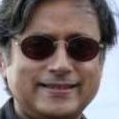
\includegraphics[width=.3\linewidth]{WithoutMask/635.png}  
  \caption{Without Mask 1}
  \label{fig:sub-first-wom}
\end{subfigure}
\begin{subfigure}{.5\textwidth}
  \centering
  % include second image
  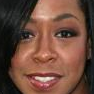
\includegraphics[width=.3\linewidth]{WithoutMask/47.png}  
  \caption{Without Mask 2}
  \label{fig:sub-second-wom}
\end{subfigure}
\caption{Without Mask Dataset Sample Figure}
\label{fig:fig}
\end{figure}
\begin{figure}[ht]
\begin{subfigure}{.5\textwidth}
  \centering
  % include first image
  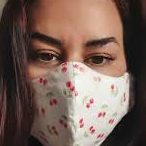
\includegraphics[width=.3\linewidth]{WithMask/53.png}  
  \caption{With Mask 1}
  \label{fig:sub-first-wm}
\end{subfigure}
\begin{subfigure}{.5\textwidth}
  \centering
  % include second image
  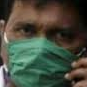
\includegraphics[width=.3\linewidth]{WithMask/85.png}  
  \caption{With Mask 2}
  \label{fig:sub-second-wm}
\end{subfigure}
\caption{With Mask Dataset Sample Figure}
\label{fig:fig}
\end{figure}
\section{Background Study}
A convolutional neural network (CNN) is a type of artificial neural network used in image recognition and processing that is specifically designed to process pixel data. The layers of a CNN consist of an input layer, an output layer and a hidden layer that includes multiple convolutional layers, pooling layers, fully connected layers and normalization layers. The removal of limitations and increase in efficiency for image processing results in a system that is far more effective, simpler to trains limited for image processing and natural language processing.
\\
\\
A residual neural network (ResNet) is a kind of deep transfer learning based on residual learning. All types of ResNet-101, ResNet-50, and ResNet-18 are versions of ResNet to get rid of the problem of vanishing gradients that have their specific residual block. ResNet-50 with 50-layers are deep, start with a convolution layer, and end with a fully-connected layer, and in between followed by 16 residual bottleneck blocks each block has three layers of convolution layer.
\\
\\
Inception-v3 is a convolutional neural network that is 48 layers deep. The Inception V3 model used several techniques for optimizing the network for better model adaptation. It has a deeper network compared to the Inception V1 and V2 models, but its speed isn't compromised. 
VGG incorporates 1x1 convolutional layers to make the decision function more non-linear without changing the receptive fields. The small-size convolution filters allows VGG to have a large number of weight layers; of course, more layers leads to improved performance.
\\
\\
The experimental trials for this work are conducted using the Google Colab environment. For evaluating the performance of our chosen models, several performance metrics are used namely Accuracy, Precision, Recall and F1 Score.

\subsection{Accuracy}
Accuracy is a metric that describes how the model performs in general across all classes. It is helpful when all classes are equally important. It is determined by dividing the number of correct predictions by the total number of predictions. Formula of Accuracy is given below:
{\begin{equation*}
    \text{Accuracy} = \frac{\text{True}_{\text{Positive}}+\text{True}_{\text{Negative}}}{\text{True}_{\text{Positive}}+\text{True}_{\text{Negative}}+\text{False}_{\text{Positive}}+\text{False}_{\text{Negative}}}
\end{equation*}}
\subsection{Precision}
The precision is calculated as the ratio of Positive samples correctly classified to the total number of Positive samples classified (either correctly or incorrectly). The precision of the model measures its accuracy in classifying a sample as positive. Formula of Precision is given below:
\begin{equation*}
    \text{Precision} = \frac{\text{True}_{\text{Positive}}}{\text{True}_{\text{Positive}}+\text{False}_{\text{Positive}}}
\end{equation*}
\subsection{Recall}
The recall is calculated as the ratio of Positive samples that were correctly classified as Positive to the total number of Positive samples. The recall of the model measures its ability to detect Positive samples. The more positive samples detected, the higher the recall. Formula of Recall is given below:
\begin{equation*}
    \text{Recall} = \frac{\text{True}_{\text{Positive}}}{\text{True}_{\text{Positive}}+\text{False}_{\text{Negative}}}
\end{equation*}
\subsection{F1 Score}
The F1-score combines a classifier's precision and recall into a single metric by taking their harmonic mean. Its primary application is to compare the performance of two classifiers. Assume classifier A has a higher recall while classifier B has a higher precision. The F1-scores for both classifiers can be used to determine which one produces better results in this case. Formula of F1 Score is given below:
{\begin{equation*}
    \text{F1 Score} =2 \times \frac{\text{Precision}\times\text{Recall}}{\text{Precision}+\text{Recall}}
\end{equation*}}


\section{Experiment}
\subsection{CNN}
To identify the face mask in this case CNN is used.There are:
\begin{itemize}
    \item 4 convolution layer followed by max-pooling layer
    \item In each layer 
        \begin{itemize}
              \item Stride: 1
               \item Padding: Valid
               \item Activation: ReLu
        \end{itemize}
    \item Then there is a flatten layer
    \item finally,there are 5 fully connected dense layer.
    \item In the output layer there are 2 outputs as it is a binary classification and activation is sigmoid and optimizer is RMSProp.
\end{itemize}

\begin{table}[htbp]
\caption{CNN}
\label{tab:cnn}
\begin{center}
\begin{tabular}{|c|c|}
\hline
\textbf{Total params}                                                   & 2,786,113 \\ \hline
\textbf{Trainable params}                                               & 2,786,113 \\ \hline
\textbf{\begin{tabular}[c]{@{}c@{}}Non-trainable\\ params\end{tabular}} & 0         \\ \hline
\textbf{Accuracy}                                                       & 97.35\%   \\ \hline
\textbf{F1-Score}                                                       & 94.34\%   \\ \hline
\textbf{Precision}                                                      & 97.32\%   \\ \hline
\textbf{Recall}                                                         & 91.79\%   \\ \hline
\end{tabular}
\end{center}
\end{table}




\subsection{Vgg16}
To identify the face mask secondly Vgg16 is used.There are:
\begin{itemize}
    \item 5 blocks followed by a pooling layer
    \item In first 2 blockes there are 2 convolutional layers
    \item rest 3 blockes have 3 convolutional layers 
    \item Finally there are 4 fully connected dense layer
     \item In the output layer there are 2 outputs as it is a binary classification and activation is sigmoid and optimizer is Adam.
    
\end{itemize}
\begin{table}[htbp]
\caption{VGG16}
\label{tab:vgg}
\begin{center}
\begin{tabular}{|c|c|}
\hline
\textbf{Total params}                                                   & 19,121,989 \\ \hline
\textbf{Trainable params}                                               & 4,407,301 \\ \hline
\textbf{\begin{tabular}[c]{@{}c@{}}Non-trainable\\ params\end{tabular}} & 14,714,688         \\ \hline
\textbf{Accuracy}                                                       & 98.79\%   \\ \hline
\textbf{F1-Score}                                                       & 51.08\%   \\ \hline
\textbf{Precision}                                                      & 51.61\%  \\ \hline
\textbf{Recall}                                                         & 50.57\%   \\ \hline
\end{tabular}
\end{center}
\end{table}

\subsection{Resnet50}
To identify the face mask thirdly resnet50 is used.There are:
\begin{itemize}
    \item 5 stages each with a convolution and Identity block. 
    \item Each convolution block has 3 convolution layers and each identity block also has 3 convolution layers.
    \item It is a variant of ResNet model which has 48 Convolution layers along with 1 MaxPool and 1 Average Pool layer.
    \item It has over 23 million trainable parameters.
    \item Finally there are 4 fully connected dense layer and ReLu as Activation.
     \item In the output layer there are 2 outputs as it is a binary classification and activation is sigmoid and optimizer is Adam.
    
\end{itemize}
\begin{table}[htbp]
\caption{RestNet50}
\label{tab:restnet}
\begin{center}
\begin{tabular}{|c|c|}
\hline
\textbf{Total params}                                                   &  40,283,013 \\ \hline
\textbf{Trainable params}                                               & 16,695,301 \\ \hline
\textbf{\begin{tabular}[c]{@{}c@{}}Non-trainable\\ params\end{tabular}} & 23,587,712        \\ \hline
\textbf{Accuracy}                                                       & 70.67\%   \\ \hline
\textbf{F1-Score}                                                       & 39.92\%   \\ \hline
\textbf{Precision}                                                      & 51.61\%   \\ \hline
\textbf{Recall}                                                         & 33.03\%   \\ \hline
\end{tabular}
\end{center}
\end{table}
\subsection{Inception-V3}
To identify the face mask thirdly Inception-V3 is used.There are:
\begin{itemize}
    \item inception-v3 is 48 layers deep. 
    \item It has a deeper network and Higher efficiency.
    \item It uses auxiliary Classifiers as regularizes.
    \item There are also 4 connected dense layer and ReLu as Activation.
     \item In the output layer there are 2 outputs as it is a binary classification and activation is sigmoid and optimizer is Adam.
    
\end{itemize}
\begin{table}[htbp]
\caption{RestNet50}
\label{tab:restnet}
\begin{center}
\begin{tabular}{|c|c|}
\hline
\textbf{Total params}                                                   & 26,210,085 \\ \hline
\textbf{Trainable params}                                               & 4,407,301 \\ \hline
\textbf{\begin{tabular}[c]{@{}c@{}}Non-trainable\\ params\end{tabular}} & 21,802,784         \\ \hline
\textbf{Accuracy}                                                       & 98.89\%   \\ \hline
\textbf{F1-Score}                                                       & 51.46\%   \\ \hline
\textbf{Precision}                                                      & 51.51\%   \\ \hline
\textbf{Recall}                                                         & 51.41\%   \\ \hline
\end{tabular}
\end{center}
\end{table}
\newpage
\subsection{Loss Accuracy Comparison}
\begin{figure}[htbp]
        \centerline{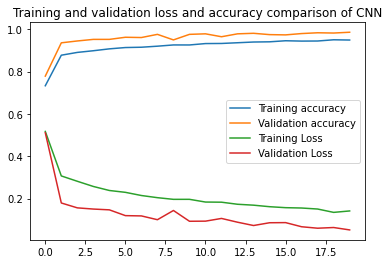
\includegraphics[width=8cm]{CNN.png}}
        \caption{CNN}
        \label{output}
    \end{figure}

\begin{figure}[htbp]
        \centerline{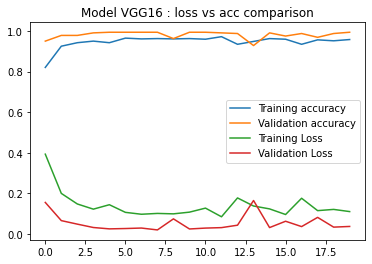
\includegraphics[width=8cm]{VGG.png}}
        \caption{VGG16}
        \label{output}
    \end{figure}
 
\begin{figure}[htbp]
        \centerline{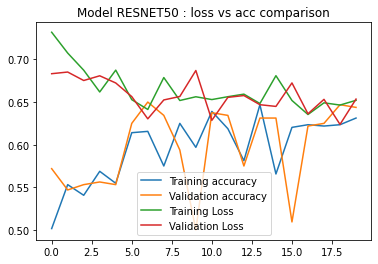
\includegraphics[width=8cm]{RESNET.png}}
        \caption{RESNET}
        \label{output}
    \end{figure}  
    
\begin{figure}[htbp]
        \centerline{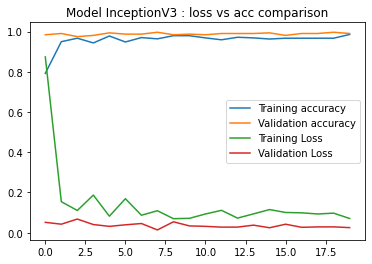
\includegraphics[width=8cm]{INCEPTION.png}}
        \caption{INCEPTION}
        \label{output}
    \end{figure}
\newpage   
\subsection{Output}



\begin{figure}[htbp]
        \centerline{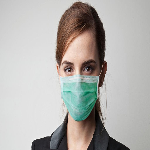
\includegraphics[width=5cm]{cnno.png}}
        \caption{CORRECT OUTPUT FROM CNN MoDEL}
        \label{output}
    \end{figure}

\begin{figure}[htbp]
        \centerline{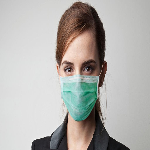
\includegraphics[width=5cm]{vggo.png}}
        \caption{CORRECT OUTPUT FROM VGG16 MoDEL}
        \label{output}
    \end{figure}
\newpage
\begin{figure}[htbp]
        \centerline{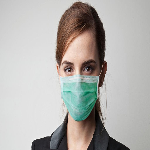
\includegraphics[width=5cm]{resneto.png}}
        \caption{CORRECT OUTPUT FROM RESNET50 MoDEL}
        \label{output}
    \end{figure}
\begin{figure}[htbp]
        \centerline{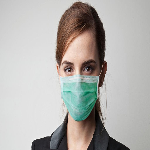
\includegraphics[width=5cm]{inceptiono.png}}
        \caption{CORRECT OUTPUT FROM INCEPTION-V3 MoDEL}
        \label{output}
    \end{figure}
\section{Result Analysis}



\begin{table}[htbp]
\caption{Summary of ALL Models}
\label{tab:summary}
\begin{tabular}{|c|c|c|c|c|}
\hline
\textbf{MODELS}             & \textbf{ACCURACY} & \textbf{F1-Score}    & \textbf{PRECISION} & \textbf{RECALL}                  \\ \hline
CNN                         &  97.35\% &            94.34\%            &      97.32\%               &      91.79\%              \\ \hline
VGG16  &  98.79\%   & 51.08\%  & 51.61\%  & 50.57\% \\ \hline
RESNET50     & 70.67\%   & 39.92\%    & 51.61\%   &  33.03\%  \\ \hline
INCEPTION-V3  & 98.89\%   & 51.46\%  & 51.51\%   & 51.41\%  \\ \hline

\end{tabular}
\end{table}

Here we can see that The accuracy of Inception-V3 and Resnet50 is almost 99\% and CNN is 97.34\%.

On the other hand F1-score, Precision, Recall are very satisfactory for CNN but it is not that much better in other models. so, from these we can decide the best model for this mask detection is CNN.

Mainly for CNN there were almost 2,786,113 parameters and here this model trained all data.On the other hand other models are unable to train all data. so, CNN gives the best result.

\newpage
So here is The Summery of our best model CNN: 




\begin{table}[htbp]
\caption{Summary of CNN Model}
\label{tab:summary}
\begin{tabular}{|c|c|c|}
\hline
\textbf{Layer (type)}             & \textbf{Output Shape} & \textbf{Param \#} \\ \hline
conv2d (Conv2D)                   & (None, 148, 148, 32)  & 896               \\ \hline
max\_pooling2d (MaxPooling2D)     & (None, 74, 74, 32)    & 0                 \\ \hline
conv2d\_1 (Conv2D)                & (None, 72, 73, 64)    & 12352             \\ \hline
max\_pooling2d\_1 (MaxPooling 2D) & (None, 36, 36, 64)    & 0                 \\ \hline
conv2d\_2 (Conv2D)                & (None, 34, 34, 128)   & 73856             \\ \hline
max\_pooling2d\_2 (MaxPooling 2D) & (None, 17, 17, 128)   & 0                 \\ \hline
conv2d\_3 (Conv2D)                & (None, 15, 15, 256)   & 295168            \\ \hline
max\_pooling2d\_3 (MaxPooling 2D) & (None, 7, 7, 256)     & 0                 \\ \hline
conv2d\_4 (Conv2D)                & (None, 5, 5, 512)     & 1180160           \\ \hline
max\_pooling2d\_4 (MaxPooling 2D) & (None, 2, 2, 512)     & 0                 \\ \hline
dropout (Dropout)                 & (None, 2, 2, 512)     & 0                 \\ \hline
flatten (Flatten)                 & (None, 2048)          & 0                 \\ \hline
dense (Dense)                     & (None, 512)           & 1049088           \\ \hline
dense\_1 (Dense)                  & (None, 256)           & 131328            \\ \hline
dense\_2 (Dense)                  & (None, 128)           & 32896             \\ \hline
dense\_3 (Dense)                  & (None, 64)            & 8256              \\ \hline
dense\_4 (Dense)                  & (None, 32)            & 2080              \\ \hline
dense\_5 (Dense)                  & (None, 1)             & 33                \\ \hline
\end{tabular}
\end{table}

\section{Future Works}
Here we tried to detect if anyone carrying mask or not. In future we will try to train our all non-trainable parameters and will attempt to detect if anyone carrying mask properly or not.

Applying different models can give better result as well.

\section{Conclusion}
It is necessary to take action to stop the COVID19 pandemic from spreading. This face mask recognition technique is an extremely effective approach to accomplish this. The ones who are not wearing masks will be separated from the crowd by the system. The ability of the face mask detection system to adjust for the benefit of the public is increased by the identification of those who violate COVID standards. The face mask detection system has the potential to ensure both our safety and the safety of others if it is used properly. This method not only aids in reaching high precision but also greatly speeds up face detection. In order to keep an eye on the crowd and make sure that everyone is wearing a mask, the system can be used in a variety of locations, including marketplaces, railroad stations, schools, and metro stations. The book is also useful for aspiring scholars and fans. In order to ensure that this model is not restricted to just face mask recognition systems, it may be employed in any high-definition camcorders. In addition, biometric scans can be performed using this when the subject is wearing a mask.
\newline
\newline
\newline
\begin{thebibliography}{00}
\bibitem{b1} Rahman, Mohammad Marufur, et al. "An automated system to limit COVID-19 using facial mask detection in smart city network." 2020 IEEE International IOT, Electronics and Mechatronics Conference (IEMTRONICS). IEEE, 2020.
\bibitem{b2} M. S. Ejaz and M. R. Islam, "Masked Face Recognition Using Convolutional Neural Network," 2019 International Conference on Sustainable Technologies for Industry 4.0 (STI), 2019, pp. 1-6, doi: 10.1109/STI47673.2019.9068044.
\bibitem{b3} Kaur, Gagandeep, Ritesh Sinha, Puneet Kumar Tiwari, Srijan Kumar Yadav, Prabhash Pandey, Rohit Raj, Anshu Vashisth, and Manik Rakhra. "Face mask recognition system using CNN model." Neuroscience Informatics (2021): 100035.
\end{thebibliography}

\end{document}
